\documentclass[11pt,a4paper]{article}

% ---- packages -----
\usepackage[a4paper,margin=2.5cm]{geometry}
\usepackage[onehalfspacing]{setspace}
\usepackage[T1]{fontenc}
\usepackage{lmodern}
\usepackage{microtype}
\usepackage{booktabs}
\usepackage{tabularray}
\UseTblrLibrary{booktabs}
\UseTblrLibrary{siunitx}
\usepackage{float}
\usepackage{graphicx}
\usepackage{amsmath, amssymb}
\usepackage{natbib}
\usepackage[hidelinks]{hyperref}
\usepackage{titlesec}
\usepackage{tikz}
\usetikzlibrary{positioning, arrows.meta}
\titlespacing*{\section}{0pt}{1.0\baselineskip}{0.4\baselineskip}
\titlespacing*{\subsection}{0pt}{0.8\baselineskip}{0.3\baselineskip}

% modelsummary helpers
\providecommand{\tinytableTabularrayUnderline}[1]{\underline{#1}}
\providecommand{\tinytableTabularrayStrikeout}[1]{\sout{#1}}

\title{\textbf{MSS (2004) Revisited:\\
       Weak Instruments and Panel-Internal Identification}}
\author{Alexander Lievens and Tobias Vanoverschelde\\
\small KU Leuven: D0S91a Advanced Applied Econometrics\\
\small Prof.\ Dr.\ Dirk Czarnitzki}
\date{May 2026}

\begin{document}
\maketitle

\begin{abstract}
\noindent
We re-examine the rainfall-instrumental-variables design of
\citet{MSS2004} using post-2005 weak-instrument diagnostics and
alternative panel identification strategies taught in our course. On
the original panel of 41 sub-Saharan African countries (1981-1999),
the rainfall first stage fails the \citet{StockYogo2005}
10\%-maximum-size critical value by a factor of seven; the 2SLS point
estimate carries the wrong sign, the Anderson-Rubin 95\%
confidence set is $[-4.41,\,7.49]$, and a cluster-bootstrap percentile
interval covers the entire interesting parameter space. Three
panel-internal identification strategies that do not rely on
rainfall: first-difference IV \citep{AndersonHsiao1981} and
difference- and system-GMM \citep{ArellanoBond1991,BlundellBond1998},
all recover the negative MSS sign, with the difference-GMM
coefficient $-0.29$ significant at the 10\% level. The data inform
the sign of the income-conflict relationship across distinct
identifying assumptions, but pin down its magnitude only loosely under
any single design available within the original panel.
\end{abstract}

% ===========================================================================
\section{Introduction}\label{sec:intro}
% ===========================================================================
Estimating the causal effect of income shocks on civil conflict is
not an estimation problem but an identification problem. OLS confounds
three biases: conflict destroys output (reverse causation), national
accounts in low-income economies are measured with error, and
persistent country traits affect both (omitted variables). No amount
of data fixes this. The effect is identified only if we can find a
source of variation in growth that is exogenous to conflict and does
not enter the conflict equation directly.

\citet{MSS2004}, henceforth MSS, proposed that source: annual rainfall
growth, used as an excluded instrument for per-capita GDP growth on a
panel of 41 sub-Saharan African countries over 1981-1999. The
identifying assumptions are that rainfall shifts agricultural output
(relevance), and that it affects conflict only through that channel
(exclusion). The paper was novel in 2004. It also predates several of
the diagnostic tools we now use to evaluate IV designs.

The MSS design has since been challenged on three grounds: the
relevance and functional form of the first stage \citep{Ciccone2011},
the credibility of an alternative price-based instrument
\citep{BrucknerCiccone2010}, and the exclusion restriction itself
\citep{Sarsons2015}. Section~\ref{sec:critiques} reviews these
critiques.

We revisit MSS with two questions. First, how much the original
rainfall design tells us about $\beta$ once modern weak-instrument
diagnostics and weak-IV-robust inference are applied to the 2SLS
output. Second, whether panel-internal identification strategies that
do not rely on rainfall, from \citet{AndersonHsiao1981}
first-difference IV to the difference- and system-GMM estimators of
\citet{ArellanoBond1991} and \citet{BlundellBond1998}, recover a
coherent estimate.

Section~\ref{sec:identification} formalises the MSS identification.
Section~\ref{sec:critiques} surveys the critiques.
Section~\ref{sec:data} describes the data. Section~\ref{sec:methods}
sets out the estimators. Section~\ref{sec:results} reports estimates.
Section~\ref{sec:discussion} concludes.

% ===========================================================================
\section{The MSS identification strategy}\label{sec:identification}
% ===========================================================================
MSS fit the structural equation
\begin{equation}
C_{it} = \alpha_i + \lambda_i t + \beta\, g^{y}_{it} + \gamma' X_{it} + u_{it},
\label{eq:structural}
\end{equation}
where $C_{it} = \mathbf{1}\{\text{conflict}_{it}\}$ is a binary indicator for civil
conflict in country $i$ at year $t$, $\alpha_i$ are country fixed effects, $\lambda_i t$ are country-specific linear time trends, $g^{y}_{it} = \Delta \log(\text{GDP}_{it})$ is per-capita GDP growth, and $X_{it}$ collects time-varying controls (lagged Polity~2). Opportunity-cost theory \citep{Grossman1991} predicts
$\beta < 0$.

Estimating equation~\eqref{eq:structural} by OLS is inconsistent for the reasons
listed in Section~\ref{sec:intro}. MSS instrument $g^{y}_{it}$ with annual
rainfall growth $g^{R}_{it}$ and its first lag:
\begin{equation}
g^{y}_{it} = a_i + b_i t + \pi_1\, g^{R}_{it} + \pi_2\, g^{R}_{i,t-1}
             + \delta' X_{it} + v_{it}.
\label{eq:firststage}
\end{equation}

The identifying assumptions, made conditional on $\alpha_i$ and $X_{it}$, are:

\textit{Relevance}: $\mathrm{Cov}(g^{R}_{it}, g^{y}_{it}) \neq 0$. Rainfall shifts
agricultural output, which is a large share of African GDP. Testable through the
first-stage $F$ statistic on the excluded instruments.

\textit{Exclusion}: $\mathrm{Cov}(g^{R}_{it}, u_{it}) = 0$. Rainfall affects
conflict only through GDP. Not directly testable in general; with two
instruments, the Sargan test provides one degree of freedom of indirect check on
whether the two rainfall measures imply the same $\beta$.

\begin{figure}[H]
\centering
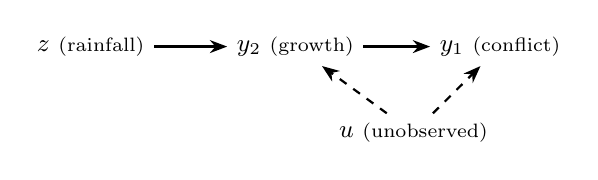
\begin{tikzpicture}[
  node distance=2.2cm,
  every node/.style={font=\small},
  arr/.style={->, >={Stealth[length=2.2mm]}, thick}
]
  \node (z)  {$z$ \scriptsize(rainfall)};
  \node[right of=z, xshift=0.4cm]  (y2) {$y_2$ \scriptsize(growth)};
  \node[right of=y2, xshift=0.4cm] (y1) {$y_1$ \scriptsize(conflict)};
  \node[below=0.6cm of y2, xshift=1.5cm] (u)  {$u$ \scriptsize(unobserved)};

  \draw[arr] (z)  -- (y2);
  \draw[arr] (y2) -- (y1);
  \draw[arr, dashed] (u) -- (y2);
  \draw[arr, dashed] (u) -- (y1);
\end{tikzpicture}
\caption{The MSS identification strategy as a DAG. Solid arrows: assumed
causal pathway ($z \to y_2 \to y_1$). Dashed arrows: unobserved
confounders that bias OLS. Identification of $\beta$ requires the
$z \to y_2$ arrow (relevance, testable) and the \emph{absence} of any
$z \to y_1$ arrow (exclusion, not directly testable).}
\label{fig:dag-mss}
\end{figure}

The specification choices matter, which is why MSS use country fixed effects to absorb time-invariant heterogeneity (geography, institutions, colonial history) and
country-specific linear time trends to absorb slow secular movements
(democratisation, technology diffusion). They do not use year fixed effects,
which would absorb the common component of rainfall shocks across the panel
and reduce the variation the instrument exploits. Standard errors are clustered
at the country level.

Their preferred 2SLS specification yields $\hat\beta \approx -2.4$: a
five-percentage-point decline in growth raises the probability of conflict by
roughly twelve percentage points.

% ===========================================================================
\section{Methodological critiques and alternative identification}\label{sec:critiques}
% ===========================================================================
The literature that followed MSS extended the design along three axes:
it offered alternative instruments, questioned the first-stage
specification, and tested the exclusion restriction directly. Only the
last two are critiques in the strict sense; the first is a parallel
identification strategy.

\textbf{Alternative instrument.} \citet{BrucknerCiccone2010} replace
rainfall with country-specific commodity export price shocks (a
weighted sum of global commodity prices using each country's export
composition as weights), instrumenting growth in the same structural
equation~\eqref{eq:structural}. The exogeneity argument is
small-country price-taking: global commodity prices are determined on
world markets, and no single sub-Saharan African country is large
enough to move them. They recover a negative and significant $\beta$,
corroborating the MSS sign under a different identifying assumption.
This is identification pluralism rather than critique: two unrelated
exogeneity arguments converge on the same conclusion, which strengthens
MSS rather than weakens it. Within MSS's own design, the analogue is
the Sargan over-identification test on the two rainfall instruments
(current and lagged); we return to it in Section~\ref{sec:results}.

\textbf{Specification critique.} \citet{Ciccone2011} attacks the
functional form rather than the exogeneity. He shows that the original
MSS result stems from a counterintuitive \emph{positive} correlation
between conflict at $t$ and rainfall levels at $t-2$, rather than from
negative rainfall shocks lowering income and raising conflict through
the agricultural channel. Re-examining the analysis with updated data,
he reports that conflict is largely unrelated to rainfall.
\citet{MiguelSatyanath2011} reply arguing that the MSS findings remain
when rainfall levels are used as instruments, while acknowledging that
the first-stage relationship weakens after 2000. The lesson is generic:
an exogenous instrument applied in the wrong functional form still
produces an inconsistent estimate.

\textbf{Direct test of exclusion.} The most consequential critique
tests the exclusion restriction itself. \citet{Sarsons2015} uses
Indian district-level data on rainfall and Hindu-Muslim religious
riots, combined with records of irrigation dams. In districts
\emph{downstream of dams}, water supply is decoupled from local
rainfall: income in these districts is much less sensitive to rainfall
fluctuations, so the agricultural channel is mechanically attenuated.
If MSS's exclusion holds (rainfall affects conflict only through
agricultural income), then in dam-downstream districts rainfall should
not predict conflict. She finds that rain shocks remain equally strong
predictors of riot incidence in downstream districts. The implication is a
direct $z \to y_1$ arrow that the MSS DAG denies (Figure~\ref{fig:dag-sarsons}).

\begin{figure}[H]
\centering
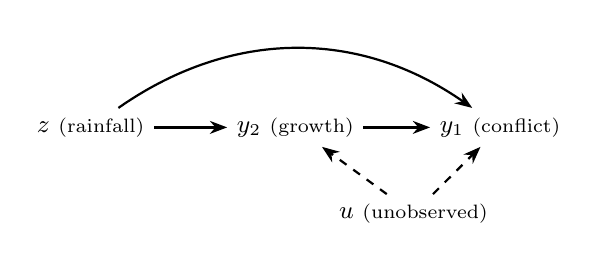
\begin{tikzpicture}[
  node distance=2.2cm,
  every node/.style={font=\small},
  arr/.style={->, >={Stealth[length=2.2mm]}, thick}
]
  \node (z)  {$z$ \scriptsize(rainfall)};
  \node[right of=z, xshift=0.4cm]  (y2) {$y_2$ \scriptsize(growth)};
  \node[right of=y2, xshift=0.4cm] (y1) {$y_1$ \scriptsize(conflict)};
  \node[below=0.6cm of y2, xshift=1.5cm] (u)  {$u$ \scriptsize(unobserved)};

  \draw[arr] (z)  -- (y2);
  \draw[arr] (y2) -- (y1);
  \draw[arr, dashed] (u) -- (y2);
  \draw[arr, dashed] (u) -- (y1);
  \draw[arr, thick] (z) to[bend left=35] (y1);
\end{tikzpicture}
\caption{Sarsons's critique as a DAG. Same as Figure~\ref{fig:dag-mss}
plus a direct $z \to y_1$ arrow that exclusion denies. Evidence from
regions where the $z \to y_2$ channel is physically blocked
(downstream of dams) supports the existence of this arrow.}
\label{fig:dag-sarsons}
\end{figure}

The methodological lesson is general. Exclusion restrictions are
sometimes partially testable: if the IV is claimed to operate through
one channel, find a setting where the channel is shut and check whether
the IV still moves the outcome. The post-2015 standard for IV papers in
development economics has internalised this test.

% ===========================================================================
\section{Data}\label{sec:data}
% ===========================================================================
{\sloppy We use the replication panel distributed by MSS via the
Harvard Dataverse (doi:10.7910/DVN/27324). It covers 41 sub-Saharan
African countries over 1981-1999. After constructing one lag of GDP
growth and dropping country-years with missing controls, the
estimation sample is 702 country-year observations.\par}

The outcome \texttt{any\_prio} is a PRIO indicator equal to one if a
country experiences at least 25 battle deaths in a year. The endogenous
regressor \texttt{gdp\_g} is annual per-capita GDP growth. The excluded
instruments are current and lagged rainfall growth, \texttt{GPCP\_g}
and \texttt{GPCP\_g\_l}, constructed from the Global Precipitation
Climatology Project. Controls follow MSS: initial log income, lagged
Polity~2, ethnic and religious fractionalisation, an oil-exporter
dummy, log mountainous terrain, and log lagged population. Only lagged
Polity~2 is time-varying; the rest are absorbed by country fixed
effects in our preferred specifications.

\begin{table}[H]
\centering
\caption{Descriptive statistics, estimation sample ($N = 702$).}
\label{tab:descriptives}
\begin{tabular}{lrrrrr}
\toprule
Variable & $N$ & Mean & SD & Min & Max \\
\midrule
\texttt{any\_prio}  & 702 & 0.269   & 0.444 & 0.000   & 1.000 \\
\texttt{gdp\_g}     & 702 & $-0.006$ & 0.066 & $-0.474$ & 0.319 \\
\texttt{GPCP\_g}    & 702 & 0.015   & 0.210 & $-0.550$ & 1.680 \\
\texttt{y\_0}       & 702 & 1.16    & 0.90  & 0.316   & 4.84  \\
\texttt{polity2l}   & 702 & $-3.55$ & 5.55  & $-10$   & 9     \\
\texttt{ethfrac}    & 702 & 0.655   & 0.237 & 0.036   & 0.925 \\
\texttt{relfrac}    & 702 & 0.487   & 0.185 & 0.000   & 0.783 \\
\texttt{Oil}        & 702 & 0.117   & 0.321 & 0       & 1     \\
\texttt{lmtnest}    & 702 & 1.58    & 1.43  & 0       & 4.42  \\
\texttt{lpopl1}     & 702 & 8.77    & 1.20  & 5.75    & 11.7  \\
\bottomrule
\end{tabular}
\end{table}

Three features of the panel matter for what follows. The unconditional
conflict frequency is 27\%. Average growth is slightly negative
($-0.6\%$ per annum). The panel is democracy-poor on average (mean
Polity~2 of $-3.5$ on a scale of $-10$ to $10$).

% ===========================================================================
\section{Methodology}\label{sec:methods}
% ===========================================================================
The estimators below differ in how aggressively they purge the
endogeneity sources of Section~\ref{sec:intro} from the structural
equation. POLS uses all variation jointly and trusts that endogeneity
bias is small. FE removes the time-invariant part of $u$. 2SLS exploits
the rainfall instrument (the $z \to y_2$ arrow in
Figure~\ref{fig:dag-mss}) and assumes no direct $z \to y_1$ arrow. The
cluster bootstrap and the Anderson-Rubin test are inference tools, not
identification strategies, and supplement 2SLS when conventional
asymptotics are unreliable. First-difference IV with lagged levels and
the dynamic-panel GMM estimators identify $\beta$ without using
rainfall at all, relying on internal panel variation instead.

\subsection{Pooled OLS (LPM)}\label{sec:pols}

We begin by estimating equation~\eqref{eq:structural} by OLS,
$\hat\beta_{\text{POLS}} = (X'X)^{-1} X' C$, treating the binary
outcome as a linear probability model. Consistency requires
$\mathrm{Cov}(g^{y}_{it}, u_{it}) = 0$, which the three endogeneity
sources in Section~\ref{sec:intro} rule out. POLS therefore serves as
a benchmark, not as a causal estimate. The LPM is heteroscedastic by
construction since $\mathrm{Var}(u \mid x) = p(x)(1-p(x))$ depends on
$x$; we report the Breusch-Pagan and White tests as confirmation, and
cluster standard errors at the country level throughout to handle
within-country correlation.

\subsection{Fixed and random effects}\label{sec:fe}

Fixed-effects estimation removes the time-invariant part of $u$. Let
$u_{it} = c_i + e_{it}$ with $c_i$ constant within country; the within
transformation subtracts country means from each variable, giving an
estimator that is consistent if $\mathrm{Cov}(g^{y}_{it}, e_{it}) = 0$
after demeaning. We report two-way FE (country and year) as our
baseline and add a specification with country-specific linear trends
in place of year FE, the original MSS choice. The two differ in how
they treat the common component of rainfall variation across the
panel: year FE absorb it, country trends preserve it. Random effects
is consistent under the stronger assumption $\mathrm{Cov}(c_i, x_{it})
= 0$ and is more efficient when it holds; the Hausman test compares
FE and RE. Time-invariant controls (initial income, fractionalisation,
terrain, oil, lagged population) are absorbed by country FE and do
not appear in the FE or RE specifications.

\subsection{Two-stage least squares}\label{sec:2sls}

We then implement the MSS strategy: instrument $g^{y}_{it}$ with
current and lagged rainfall growth from equation~\eqref{eq:firststage},
obtain fitted values $\hat g^{y}_{it}$ from the first stage, and plug
them into the structural equation. Two assumptions support
consistency.

\textit{Relevance.} We test it through the cluster-robust $F$ statistic
on the excluded instruments in the first stage \citep{StaigerStock1997},
compared to the \citet{StockYogo2005} 10\%-maximum-size critical value
of 19.93 (two IVs, one endogenous regressor). Values below the
threshold indicate weak instruments and invalid conventional standard
errors.

\textit{Exclusion.} Not directly testable. With two instruments we
report the Sargan over-identification test, which asks whether both
rainfall measures imply the same $\beta$. Rejection indicates that at
least one instrument is correlated with $u$. Failure to reject is weak
evidence at best given the single degree of freedom and the fact that
both instruments share the same exogeneity argument; the test cannot
detect homogeneous invalidity.

We additionally report the Wu-Hausman endogeneity test, which compares
OLS and 2SLS and rejects exogeneity of $g^{y}_{it}$ if the two
estimates differ by more than sampling noise. Failure to reject can
equally well reflect low power: under a weak instrument the 2SLS
estimate becomes so imprecise that the test cannot detect any
systematic difference from OLS.

\subsection{Cluster bootstrap and weak-IV-robust inference}\label{sec:boot}

When the first-stage $F$ falls short of conventional critical values,
the standard 2SLS $t$-statistic does not have an asymptotic standard
normal distribution and reported confidence intervals can have actual
coverage far below their nominal level. We supplement the conventional
output with two robust procedures. The first is a non-parametric
cluster bootstrap: countries are resampled with replacement, the 2SLS
coefficient is re-estimated on each resampled panel, and the percentile
interval is reported from $B = 500$ replications. Resampling at the
country level preserves the within-country correlation structure that
cluster-robust standard errors assume.

The second is the \citet{AndersonRubin1949} test, which is the
theoretically correct route under genuinely weak instruments. It tests
$H_0\colon \beta = \beta_0$ by checking whether the instruments still
have explanatory power in the reduced form once $\beta_0$ is imposed;
the resulting confidence set has correct coverage under arbitrarily
weak first stages. We invert the test on a fine grid to obtain the 95\%
confidence set for $\beta$.

\subsection{First-difference IV with lagged levels}\label{sec:ahiv}

If rainfall is too weak to identify $\beta$ externally, the panel
itself contains a second source of variation. First-differencing
equation~\eqref{eq:structural} eliminates the country fixed effects:
\[
\Delta C_{it} = \beta\, \Delta g^{y}_{it} + \gamma' \Delta X_{it}
              + \Delta u_{it}.
\]
\citet{AndersonHsiao1981} propose instrumenting the differenced
regressor $\Delta g^{y}_{it}$ with its lagged level $g^{y}_{i,t-1}$,
under the assumption $\mathrm{Cov}(g^{y}_{i,t-1},\Delta u_{it}) = 0$:
past growth is uncorrelated with the change in unobserved conflict
shocks. This identifying assumption is logically separate from the
rainfall exclusion restriction; the two strategies fail or succeed for
different reasons. With a single instrument the design is exactly
identified, so the Sargan test does not apply; the Wu-Hausman
diagnostic from Section~\ref{sec:2sls} still does.

\subsection{Difference and system GMM}\label{sec:gmm}

Conflict is highly persistent: the lagged outcome is a strong predictor
of current conflict. Extending equation~\eqref{eq:structural} with
$C_{i,t-1}$ as a regressor turns it into a dynamic panel,
\begin{equation}
C_{it} = \alpha_i + \rho\, C_{i,t-1} + \beta\, g^{y}_{it}
       + \gamma' X_{it} + u_{it}.
\label{eq:dynamic}
\end{equation}
\citet{ArellanoBond1991} first-difference equation~\eqref{eq:dynamic}
to eliminate $\alpha_i$ and instrument the differenced lagged outcome
$\Delta C_{i,t-1}$ with deeper lags of the level outcome $C_{i,t-2},
C_{i,t-3}, \ldots$; the endogenous $\Delta g^{y}_{it}$ is instrumented
similarly. \citet{BlundellBond1998} extend this with additional moment
conditions on the levels equation (system-GMM), more efficient when
the series are persistent. We use two-step estimators with
cluster-robust SE and collapse the instrument matrix to lags two and
three to keep the instrument count well below $N = 41$
\citep{Roodman2009}. Validity is assessed via the Sargan-Hansen test
on the over-identifying restrictions and the Arellano-Bond $m_2$ test
for second-order autocorrelation in the differenced residuals; failure
to reject $m_2$ is a necessary condition for the moment conditions to
hold.

% ===========================================================================
\section{Results and diagnostics}\label{sec:results}
% ===========================================================================
Table~\ref{tab:main} reports the seven static specifications described
in Section~\ref{sec:methods}. Table~\ref{tab:diag} reports the
diagnostic battery and Table~\ref{tab:ah} the panel-internal
identification strategies (Anderson-Hsiao, Arellano-Bond,
Blundell-Bond).

\begin{table}[H]
\centering
\caption{Static specifications. Cluster-robust SE at country level in
parentheses. Models 2-6 use two-way FE; model~7 replaces year FE with
country-specific linear time trends. Time-invariant controls are
included in POLS only and absorbed by country FE elsewhere.}
\label{tab:main}
\small
\begin{tabular}{lrrrrrrr}
\toprule
 & POLS & FE & RE & Red.\ form & First stage & 2SLS & 2SLS \\
 & (LPM) & 2-way & 2-way & & & & (trends) \\
\midrule
GDP growth        & $-0.507^{**}$ & $-0.460^{**}$ & $-0.443^{**}$ &        &              & $0.141$       & $-1.297$ \\
                  & $(0.222)$     & $(0.220)$     & $(0.217)$     &        &              & $(1.330)$     & $(1.071)$ \\
GDP growth (lag)  & $0.020$       & $-0.173$      & $-0.121$      &        &              & $-0.165$      & $0.040$ \\
                  & $(0.243)$     & $(0.221)$     & $(0.277)$     &        &              & $(0.229)$     & $(0.185)$ \\
Rainfall growth   &               &               &               & $0.024$ & $0.042^{**}$ &              &  \\
                  &               &               &               & $(0.055)$ & $(0.018)$  &              &  \\
Rainfall growth (lag) &           &               &               & $-0.084^{*}$ & $0.025$ &              &  \\
                  &               &               &               & $(0.048)$ & $(0.016)$  &              &  \\
Polity~2 (lag)    & $0.000$       & $-0.004$      & $-0.002$      & $-0.003$ & $-0.001^{*}$ & $-0.003$    & $-0.004$ \\
                  & $(0.004)$     & $(0.005)$     & $(0.005)$     & $(0.005)$ & $(0.001)$   & $(0.006)$   & $(0.005)$ \\
\midrule
$N$               & 702 & 702 & 702 & 702 & 702 & 702 & 702 \\
$R^2$             & 0.129 & 0.012 & 0.006 & 0.005 & 0.019 & 0.569 & 0.710 \\
\bottomrule
\end{tabular}\\[2pt]
\footnotesize $^{*}p<0.1$, $^{**}p<0.05$, $^{***}p<0.01$.
\end{table}

POLS reproduces the MSS direction: a one-standard-deviation drop in
growth ($\approx 6.6$ percentage points) raises the conflict
probability by $0.51 \times 0.066 \approx 3.4$ percentage points,
significant at the 5\% level. FE and RE shrink the coefficient slightly
towards zero ($\hat\beta = -0.46, -0.44$) with widened standard errors,
as expected when between-country variation is stripped out. The reduced
form shows that rainfall growth enters the conflict equation only
weakly (lagged rainfall has $p = 0.08$). The first stage confirms that
current-year rainfall growth has a statistically significant but
quantitatively modest effect on GDP growth.

The 2SLS estimate (column 6) is the striking column. The point estimate
is $+0.14$ with a cluster-robust SE of $1.33$: the wrong sign, no
statistical significance, and a confidence interval covering essentially
all economically relevant magnitudes. This collapse of the IV estimate
relative to the well-determined POLS estimate is the canonical
fingerprint of a weak instrument. Column~7 re-estimates the same model
with country FE plus country-specific linear time trends (the MSS
specification) and recovers $\hat\beta = -1.30$ (SE $1.07$, $p = 0.23$):
the correct sign, larger in magnitude than the original MSS estimate of
$\approx -2.4$ but still imprecisely estimated. The qualitative
direction of MSS is therefore sensitive to whether secular
country-level trends are modelled.

\begin{table}[H]
\centering
\caption{Specification and identification diagnostics.}
\label{tab:diag}
\small
\begin{tabular}{lrr}
\toprule
Statistic & Value & $p$-value \\
\midrule
\textit{Heteroscedasticity} & & \\
Breusch--Pagan                                       & $142.52$ & $<10^{-16}$ \\
\textit{Panel structure} & & \\
$F$-test country FE ($H_0\colon c_i=0$)              & $14.90$  & $<10^{-16}$ \\
Hausman FE vs RE                                     & $0.04$   & $0.998$ \\
\textit{Weak instruments} & & \\
First-stage $F$ baseline (cluster-robust)            & $2.89$   & $0.056$ \\
First-stage $F$ MSS-trends (cluster Wald)            & $4.45$   & $0.012$ \\
First-stage $F$ MSS-trends (homoscedastic)           & $7.48$   & $0.0006$ \\
Stock--Yogo 10\%-maximum-size critical value         & $19.93$  & --- \\
\textit{Endogeneity} & & \\
Wu--Hausman                                          & $0.14$   & $0.705$ \\
\textit{Overidentification} & & \\
Sargan                                               & $2.40$   & $0.121$ \\
\textit{Weak-IV-robust and bootstrap inference} & & \\
Anderson--Rubin 95\% CI for $\beta^{\text{IV}}$      & $[-4.41,\,7.49]$ & --- \\
Cluster-bootstrap 95\% CI for $\beta^{\text{IV}}$    & $[-3.52,\,3.51]$ & --- \\
\bottomrule
\end{tabular}
\end{table}

The diagnostics tell a coherent story. Heteroscedasticity is decisively
present, confirming the necessity of robust standard errors for the LPM.
Country fixed effects are jointly significant, but the Hausman test
returns a vanishing statistic that we discount: the test's construction
assumes the FE estimator is efficient under $H_0$, which fails once
standard errors are clustered, and its power is limited in moderately
unbalanced panels. We default to FE.

The weak-instrument diagnostics are the crux. The first-stage $F$ on
the two excluded rainfall instruments is $2.89$ in our baseline,
roughly one-seventh of the Stock-Yogo threshold of $19.93$. The
MSS-trends specification raises it to $4.45$ (cluster-robust) or $7.48$
(homoscedastic), notably stronger but still below the threshold.
Conventional 2SLS inference is therefore unreliable in both
specifications, and the Wu-Hausman test fails to reject exogeneity
($p = 0.705$): in this sample we have no positive statistical evidence
that OLS is biased, though theory says it must be.

Under genuinely weak instruments only weak-IV-robust inference is
valid. The Anderson-Rubin 95\% confidence set for $\beta$ is
$[-4.41,\,7.49]$, uninformative about either sign or magnitude. A
non-parametric cluster bootstrap (500 replications, resampling
countries with replacement) yields a closely comparable 95\% percentile
interval of $[-3.52,\,3.51]$. The Sargan test on the two rainfall
instruments fails to reject ($p = 0.121$), which we read as weak
reassurance only.

\begin{table}[H]
\centering
\caption{Panel-internal identification strategies. Column 1 is the
\citet{AndersonHsiao1981} FD-IV on the static structural equation;
columns 2 and 3 are two-step difference- and system-GMM on the dynamic
specification~\eqref{eq:dynamic}, with collapsed instrument matrices
at lags 2--3. Cluster-robust SE at country level in parentheses.}
\label{tab:ah}
\small
\begin{tabular}{lrrr}
\toprule
 & Anderson--Hsiao & Arellano--Bond & Blundell--Bond \\
\midrule
Conflict (lag)               &              & $0.334^{**}$  & $0.628^{***}$ \\
                             &              & $(0.142)$     & $(0.095)$     \\
GDP growth                   & $-0.349$     & $-0.293^{*}$  & $-0.296$      \\
                             & $(0.383)$    & $(0.150)$     & $(0.225)$     \\
GDP growth (lag)             &              & $0.044$       & $-0.046$      \\
                             &              & $(0.211)$     & $(0.225)$     \\
Polity~2 (lag)               & $-0.005$     & $0.000$       & $-0.006^{*}$  \\
                             & $(0.005)$    & $(0.004)$     & $(0.003)$     \\
\midrule
$N$ (country-years)          & 620          & ---           & ---           \\
First-stage $F$ on $g^{y}_{i,t-1}$ & 451.7  & ---           & ---           \\
Sargan--Hansen $p$           & ---          & $0.51$        & $0.09$        \\
$m_2$ (AR(2)) $p$            & ---          & $0.50$        & $0.47$        \\
\bottomrule
\end{tabular}\\[2pt]
\footnotesize $^{*}p<0.1$, $^{**}p<0.05$, $^{***}p<0.01$.
\end{table}

The three estimators tell a consistent qualitative story under
identifying assumptions that differ. Anderson-Hsiao gives
$\hat\beta_{AH} = -0.349$ with cluster-robust SE $0.383$. The
first-stage $F$ on the lagged level $g^{y}_{i,t-1}$ is $451.7$, far
above the Stock-Yogo 10\%-maximum-size critical value of $16.4$ for
one instrument and one endogenous regressor; but the strength reflects
mean reversion in the country-level growth series rather than new
identifying variation, since high past growth predicts a large negative
change in current growth almost mechanically. Identification rests on
$\mathrm{Cov}(g^{y}_{i,t-1}, \Delta u_{it}) = 0$, which is logically
independent from the rainfall exclusion.

The Arellano-Bond difference-GMM estimator, which adds $C_{i,t-1}$ to
the equation and uses deeper lags as instruments, returns
$\hat\beta_{AB} = -0.293$ ($p \approx 0.05$). Blundell-Bond yields a
similar point estimate $-0.296$ but the standard error widens and
significance drops below the 10\% level. The lagged conflict
coefficient is large and highly significant in system-GMM
($\hat\rho = 0.628$, $p < 0.001$), confirming substantial persistence
and indicating that the static specifications of
Table~\ref{tab:main} are mis-specified. The Sargan-Hansen tests do
not reject for either estimator ($p = 0.51$ for AB; $p = 0.09$ for BB,
borderline and read with caution); the $m_2$ tests do not detect
second-order autocorrelation in differences ($p = 0.50$ and $0.47$).
Both validations support the identifying restrictions.

Across all three panel-internal designs the MSS sign reappears,
though the magnitude is pinned down only loosely. None of these
strategies uses rainfall.

\newpage

% ===========================================================================
\section{Discussion}\label{sec:discussion}
% ===========================================================================
The empirical findings are mixed and depend on identification assumptions.

OLS recovers the qualitative MSS direction with a tight standard
error: $\hat\beta_{\text{POLS}} = -0.507$. Under exogeneity of growth,
this would be the most precise summary of the conditional relationship
between growth and conflict. As a causal estimate, it is not
defensible: the three endogeneity sources of Section~\ref{sec:intro}
rule out the required orthogonality.

Under the MSS rainfall identification, conventional inference is
unreliable. The first-stage $F$ of $2.89$ in our two-way FE
specification is roughly one-seventh of the Stock-Yogo threshold; the
2SLS point estimate carries the wrong sign and the Anderson-Rubin
95\% confidence set $[-4.41,\,7.49]$ is uninformative about either
sign or magnitude. Restoring the MSS country-trend specification
raises the first stage to $4.45$ and recovers $\hat\beta = -1.30$, of
the correct sign but still imprecisely estimated. The cluster
bootstrap interval $[-3.52,\,3.51]$ confirms the order of magnitude of
the irreducible uncertainty under conventional 2SLS, though it does
not itself restore identification under weak instruments.

Under the panel-internal identification strategies of
Sections~\ref{sec:ahiv} and~\ref{sec:gmm}, the negative sign reappears
across all three estimators ($\hat\beta_{\text{AH}} = -0.349$,
$\hat\beta_{\text{AB}} = -0.293$, $\hat\beta_{\text{BB}} = -0.296$),
with Arellano-Bond significant at the 10\% level. The
Anderson-Hsiao first-stage strength is mechanical, driven by mean
reversion in growth, but the GMM estimators rest on deeper
lag-orthogonality and (for system-GMM) initial-condition restrictions
that are logically distinct from the rainfall exclusion.

The data therefore support the qualitative sign of the MSS effect
across at least two distinct identifying assumptions (rainfall
exclusion, past-growth orthogonality), but do not support a precise
magnitude or a credible defence of either assumption against the
\citet{Sarsons2015} critique, which targets the rainfall channel
directly. The Sargan over-identification test on the two rainfall
instruments does not reject, but with one degree of freedom and two
instruments that share their exogeneity argument it has neither the
power nor the structure to detect the kind of violation that matters.
A precise causal estimate of how much income shocks raise the
probability of civil conflict in this sample requires a stronger
instrument: the commodity-price approach of
\citet{BrucknerCiccone2010} being the leading candidate, or a
research design that does not rely on rainfall at all.

\newpage
% ---------------------- bibliography ----------------------
\renewcommand{\refname}{References}
\begin{thebibliography}{99}\small

\bibitem[Anderson and Hsiao(1981)]{AndersonHsiao1981}
Anderson, T.W., and C.\ Hsiao (1981). ``Estimation of dynamic models
  with error components.'' \emph{Journal of the American Statistical
  Association} 76(375): 598--606.

\bibitem[Anderson and Rubin(1949)]{AndersonRubin1949}
Anderson, T.W., and H.\ Rubin (1949). ``Estimation of the parameters
  of a single equation in a complete system of stochastic equations.''
  \emph{Annals of Mathematical Statistics} 20(1): 46--63.

\bibitem[Arellano and Bond(1991)]{ArellanoBond1991}
Arellano, M., and S.\ Bond (1991). ``Some tests of specification for
  panel data: Monte Carlo evidence and an application to employment
  equations.'' \emph{Review of Economic Studies} 58(2): 277--297.

\bibitem[Blundell and Bond(1998)]{BlundellBond1998}
Blundell, R., and S.\ Bond (1998). ``Initial conditions and moment
  restrictions in dynamic panel data models.''
  \emph{Journal of Econometrics} 87(1): 115--143.

\bibitem[Br\"uckner and Ciccone(2010)]{BrucknerCiccone2010}
Br\"uckner, M., and A.\ Ciccone (2010). ``International commodity
  prices, growth and the outbreak of civil war in Sub-Saharan Africa.''
  \emph{Economic Journal} 120(544): 519--534.

\bibitem[Ciccone(2011)]{Ciccone2011}
Ciccone, A.\ (2011). ``Economic shocks and civil conflict: A
  comment.'' \emph{American Economic Journal: Applied Economics}
  3(4): 215--227.

\bibitem[Grossman(1991)]{Grossman1991}
Grossman, H.I.\ (1991). ``A general equilibrium model of
  insurrections.'' \emph{American Economic Review} 81(4): 912--921.

\bibitem[Miguel et al.(2004)]{MSS2004}
Miguel, E., S.\ Satyanath, and E.\ Sergenti (2004). ``Economic
  shocks and civil conflict: An instrumental variables approach.''
  \emph{Journal of Political Economy} 112(4): 725--753.

\bibitem[Miguel and Satyanath(2011)]{MiguelSatyanath2011}
Miguel, E., and S.\ Satyanath (2011). ``Re-examining economic shocks
  and civil conflict.'' \emph{American Economic Journal: Applied
  Economics} 3(4): 228--232.

\bibitem[Roodman(2009)]{Roodman2009}
Roodman, D.\ (2009). ``A note on the theme of too many instruments.''
  \emph{Oxford Bulletin of Economics and Statistics} 71(1): 135--158.

\bibitem[Sarsons(2015)]{Sarsons2015}
Sarsons, H.\ (2015). ``Rainfall and conflict: A cautionary tale.''
  \emph{Journal of Development Economics} 115: 62--72.

\bibitem[Staiger and Stock(1997)]{StaigerStock1997}
Staiger, D., and J.H.\ Stock (1997). ``Instrumental variables
  regression with weak instruments.'' \emph{Econometrica} 65(3):
  557--586.

\bibitem[Stock and Yogo(2005)]{StockYogo2005}
Stock, J.H., and M.\ Yogo (2005). ``Testing for weak instruments in
  linear IV regression.'' In: \emph{Identification and Inference for
  Econometric Models: Essays in Honor of Thomas Rothenberg}, ed.\
  D.W.K.\ Andrews and J.H.\ Stock, Cambridge University Press,
  80--108.

\end{thebibliography}

\end{document}
